\chapter{Evaluation}
\label{cha:evaluation}

The design for a DIDComm-enabled ActivityPub protocol for federated social networks strives to take advantage of the features that both DIDs and DIDComm provide. The following chapter evaluates the proposed design to assess the achievement level of these features. In addition, the evaluation compares the state-of-the-art ActivityPub implementation, the extended versions mentioned in \ref{sec:extending_activitypub} and the proposed design.

\section{Decentralization}
\subsection{Trust Encryption}
ActivityPub relies on HTTPS to provide confidentiality and data integrity. This comprises a dependence on the authority issuing the certificates that make the TLS/SSL encryption possible. By implementing DIDComm, the encryption trust gets transferred to the decentralized identifiers. Thus removing dependence from any third parties. By using a nested JWT in the proposed design, a signature and encryption layer were provided. The trust in these extra layers relied solely on the DIDs communicating, and no other party was needed to ensure it. 

However, the deeply nested use of HTTPS in Mastodon's codebase did not allow testing communication using only HTTP. In addition, taking advantage of DIDComm's transport independence was not possible, due to the complexity of Mastodon. Therefore, the foundation to use any communication method with DIDComm was set, but no actual implementation could be reached.
 

\subsection{Resolving Process}
The current implementation of Mastodon relies on the Webfinger protocol, which itself relies on the DNS, to resolve \emph{username@domain} usernames to an actor object. The DNS builds the foundation of daily Internet activity. As a centralized service, being so involved in the critical part of the Internet makes it a valuable target for attacks \cite{carli2003security}. A single institution controls it, the ICANN\footnote{https://www.icann.org/}, that until 2016 was under the control of one single country \cite{lee_2016}. 
By integrating ledger-based DIDs, this dependency on Webfinger and the DNS was only partially removed. Resolving a DID does not require the DNS to be successful. However, the service endpoint in the DID document still includes the domain of the Mastodon instance where it resides. To retrieve the actor object of the user being looked up, an HTTP GET request to the service endpoint is necessary. This means that a DNS resolution will still take place. On the contrary, the approach of the coauthors of ActivityPub and the DIDs mentioned in \ref{sec:extending_activitypub} completely removes the DNS dependency by using The Onion Router \emph{(Tor)} to host the ActivityPub server \cite{webber_sporny_2017}. This indicates that if Mastodon were running in a DNS-free space, the design would achieve a fully-decentralized resolving process. 
 
\subsection{Identity Management} \label{ev:idm}

As mentioned in \ref{cha:introduction}, Mastodon uses basic password authentication to create accounts. With this, the account is restricted to a specific server. The user has no other way to register to a different server, and the identity lives as long as the instance keeps running. On the contrary, in the proposed design, the use of DIDs brings an SSI approach where the user creates his identity independently from Mastodon. In the design, the DIDs are anchored to a test network of Ethereum. Consequently, their existence and validity will persist even if the Mastodon instance ceases to exist, eliminating the \emph{single-point-of-failure} of the identity itself. On the downside, as proved in this thesis, modifying a DID document can present complications depending on the DID method. Modifications could also imply costs when not using test blockchain networks. All of this presents extra overhead for the average user, reducing the usability of such a design. Nonetheless, independent of the overhead, with the proposed design Mastodon was interoperate with an SSI ecosystem. 

\section{Security}
Mastodon implemented HTTP Signatures to add non-repudiation and preserve integrity against tampering with the messages sent within the federation. This approach fulfills the same goals as the JWS token used in the proposed design. Both methods follow the same idea and use public key cryptography to perform the signature. Furthermore, the same key generation algorithm is being used by both. Nonetheless, the downside of HTTP signatures is that they are limited to the HTTP protocol, whereas the JWS has no constraints. 
Moreover, the JSON-LD signatures provide an HTTP-independent manner to provide non-repudiation. However, the superiority of one over the other is still an open discussion \footnote{https://w3c.github.io/vc-imp-guide/\#benefits-of-json-ld-and-ld-proofs}. JSON-LD signatures offer more flexibility and thus scalability for global decentralized networks due to their compatibility with JSON-LD. In contrast, JWTs provide a straightforward way to express data with low overhead \cite{chadwick_longley_sporny_terbu_zagidulin_zundel_2022}. As Mastodon only implements them in particular cases, it is not possible to reach a verdict. 
For this thesis, the conclusion is that both the Mastodon and the proposed implementation offer the same level of non-repudiation when using HTTP as the transport protocol. 

\section{Privacy}
The user has no control over his data by using centralized identity management. DIDs, on the other hand,  implement natively the 7 Foundational Principles of \emph{Privacy by Design} \cite{cavoukian_2006}. This gives consumers control over their personal information, including choosing what to disclose and what not. \cite{sporny_longley_sabadello_reed_steele_2021}. The proposed design requires the profile URL of the user to be included in the DID document to allow the decentralized discovery of his actor object. Although the parameter inside the profile URL does not include the user's personal information, like a human-friendly username, anyone can still access this endpoint and get all the information from the actor object. This endpoint raises a significant privacy concern and opens the question of how to be discoverable while keeping privacy. A possibility could be adding the inbox URL instead of the profile URL in the DID document. This possibility would provide a direct endpoint to interact via ActivityPub with the user. This approach might prove to be better than the proposed design, not only by improving privacy but also by shortening the number of requests needed to resolve an account and find the inbox URL for the use case defined in \autoref{section:use_case}. Nonetheless, there are many other use cases where having just the inbox URL might be limiting. For example, when \emph{Alice} wants to follow \emph{Bob}. An extra service endpoint with the \emph{follow} URL would be necessary to achieve this with the same approach, and so on with other endpoints until we get to the same approach of Webber and Sporny, mentioned in \autoref{sec:extending_activitypub}. 


\section{Confidentiality}\label{sec:confidentiality}
As explained before, the only confidentiality provided by Mastodon's implementation is the use of HTTPS. By enabling DIDComm, it is possible to encrypt the payload before sending it and decrypt it after it has arrived at its target server, extending the scope of confidentiality beyond the transport layer. Theoretically, only the DIDs at the respective endpoints could see the plain text message. 
Nonetheless, the confidentiality level reached by DIDComm and the JWE standard in the proposed design has not yet achieved complete end-to-end encryption. The reason is that the Mastodon instance must have access to the private key of the DID subject to decrypt the payload and display the message to the user, as mentioned in the DIDComm requirements in \autoref{section:enabling_didcomm}. This imposes a significant risk because the private key is no longer under the user's control. The administrator of the Mastodon instance would have access to the plain-text private key, and some security countermeasures like key rotation would not be able to counter this.



\section{Usability}
The standard username format in Mastodon is compact, human-readable, and suitable to use in a social network context. As a consequence of Zooko's triangle, DIDs are not human-meaningful by design \cite{wilcox-o'hearn_2001} \cite{sporny_longley_sabadello_reed_steele_2021}. Due to the long format of a DID, it proved to be difficult to read interactions with other users when a DID is present, and mentioning a user with the DID would take a significant amount of the 500-character limit. A workaround was to use the \emph{displayName} property of the actor object, allowing a human-meaningful descriptor for a user, as shown in figure \ref{fig:did_toot}.

Furthermore, the overhead mentioned in \ref{ev:idm} to create and update a DID contributes to a less user-friendly experience, that could keep users in easy-to-use centralized services. 


\begin{figure}[H]
  \centering
  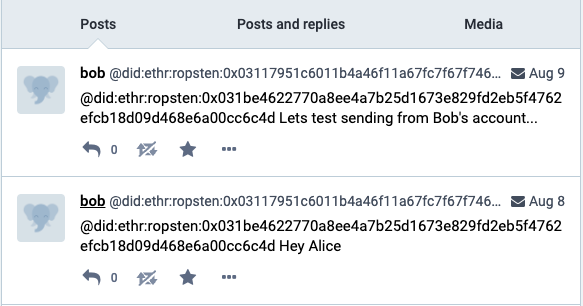
\includegraphics[width=0.8\textwidth]{evaluation/did_toot_2.png}
  \caption{Example of mentioning another user in a \emph{toot} using DIDs.}
  \label{fig:did_toot}
\end{figure}